\section{General Pupropose Processors}

GPP - generic architecture valid for a range of application fields
Common in PC/PDA
For embedded systems low end when energy and performance are not crucial and the nature of the application is quite heterogeneous.
Control and management of a slow interfacing with sensors, interactivity via GUI.
GPPs can have different architectures: 
\begin{itemize}
    \item CISC: huge amount of complex instructions. 
    \item RISC: few simple instructions
\end{itemize} 

\subsection{CISC GPP}
Ideally, each Arith/Logic operation should be capable to access (read) data and write the result by exploiting any of the available addressing modes.
Fully orthogonal architecture and Instruction Set.
In the reality, the number of operation-addressing mode combinations has been limited.
Usually one of the operand refers to the memory, while the other is a register with the role of both source and destination.
Despite this simplification, CISC instructions are coded in variable length formats. 
More complex fetch and decode units and need of more speed when accessing the memory.

\paragraph*{Architecture}
The ALU, is implementing a variety of the basic operations: Add/Sub, mul, div, logic operations, shift, comparison
In some architectures the instructions can be vectorial, working on more registers at the same time, so this is a Single Instruction Multiple Data architecture.
So many addressing mode and A/L operations, require a complex data-path that is hard to make fast. 

To increase the throughput, the CISC processors implement complex pipeline (e.g. up to 23 stages) that are hard to manage
Another strategy, still very costly in terms of hw resources, is based on altering the order of execution of the assembly instruction without modifying the semantics of the program.
For a compiler, when considering so complex pipelines, it is hard to control the status of the execution of the instruction.
The instructions could arrive to the decoding in an order that is not optimal w.r.t. the status of the pipelines at that time
Modern CISCs have dedicated hw units to dynamically reschedule the instructions
Out-of-order execution 

CISC have remarkable performance but, over the time, energy efficiency and cost moved in favor of other architectures.

\subsection{RISC GPP}
Restricted Instruction Set Computer, when the
architecture has few simple instructions.
End of '80 the price of DRAMs fall down
Size of the program is no longer a wall
CISC operations can be decomposed into RISC instructions to simplify the architecture
In the same period the integration scale raised up, dramatically
Possibility to realize on a single chip complex architectures
Pipeline and quantity of GP registers
To exploit pipelining, the execution time of the instructions must be uniform. 
This is possible when instructions are simple

Main advantage is simple instructions set and simple architecture
Instruction decoding is simplified
Frequently RISC instruction have fixed lengths
Easy balancing the stages of the pipeline and to increase clock
Execution units (ALU and BPU) take advantage from simple inst
RISC operates only on registers hence more speed and duration is predictable
RISC processor tends to have many registers, so the presence of memory spill is reduced significantly

I/O, namely load/store from memory/registers and viceversa
Each instruction requires to pre-load of the date and, eventually, to write the result in memory: load/store architecture
Data transfer operation are crucial for performance
Fortunately, the instructions have a limited number and simple of addressing modes
Aggressive use of memory (cache) hierarchy to reduce the access time to data

Software development flow
Considering the same high level source code, the number of RISC instructions will be higher that CISC
RISC architectures has no hw units to solve pipeline conflicts
But good predictability of execution allow the compiler to generate efficient code
Power consumption: RISC are simple and inherently low power w.r.t. CISC

\subsection{Superscalar GPP}
There exists a lot of parallelism at the level of assembly instruction.
It is superscalar an architecture having more than one executing units, hence more ALUs and or BPU.

The parallelism offered by the execute stage allows to deliver more instruction per clock cycle.
The complexity of the control logic increases as the impact on clock speed and power consumption. 
Moreover, it is the microprocessor to define dynamically the scheduling of the instructions. 
Pros: compiler has not to work on organizing the code for a specific hardware structure
Cons: a relevant part of the processor is deserved to implement complex scheduling mechanisms and to manage the consistency

\subsection{CISC and RISC GPP}
Approach combining out-of-order execution and superscalarity with the goal to remain compatible with code developed in the past. 
Instruction set x86 is the standard de-facto for CISC
Each CISC instruction is decomposed in a set of simple instructions easy to be executed by a simple and efficient core.
There is an hardware cost, but this solution joins the benefit of backward compatibility with the high-performance achievable by a RISC core. 

\subsection{VLIW GPP}
To overcome the limits related to the complexity of the hw scheduling of the instructions, Intel developed in the past a new class of processors named EPIC (or VLIW). 
Itanium has been the first commercialized. 
These architectures support explicit parallelism: possibility to execute more instructions at the some time under the control of the program. 
A VLIW instruction is the packing of more elementary instructions, typically RISC, in a single wide word, having a fixed structure.

The VLIW word, once fetched from the memory, is decoded in parallel.
At the end of the decoding, the single RISC instructions corresponding to the various slots, are dispatched to the different execution units.
This fixed structures moves to the compiler the task to perform a complex scheduling.
The algorithms to be optimized should be well structure to fit well a specific architecture.

EPIC/VLIW has the goal to move the complexity of the scheduling and code optimization towards the compiler.
The architectures are simple, even if of large size given the number of execution units.
Power consumption is in between simple and superscalar RISC
Similar solutions, allowing to achieve peak performance, has been adopted also in non general purpose architecture like the digital signal processors (DSPs).

\subsection{CISC and VLIW GPP}
Similar to CISC/RISC, performance of VLIW with the goal of backward compatibility.
CISC instructions are decomposed in terms of basic ones execute by a VLIW (simple and efficient) core.

\subsection{Comparison}
\begin{figure}[H]
    \centering
    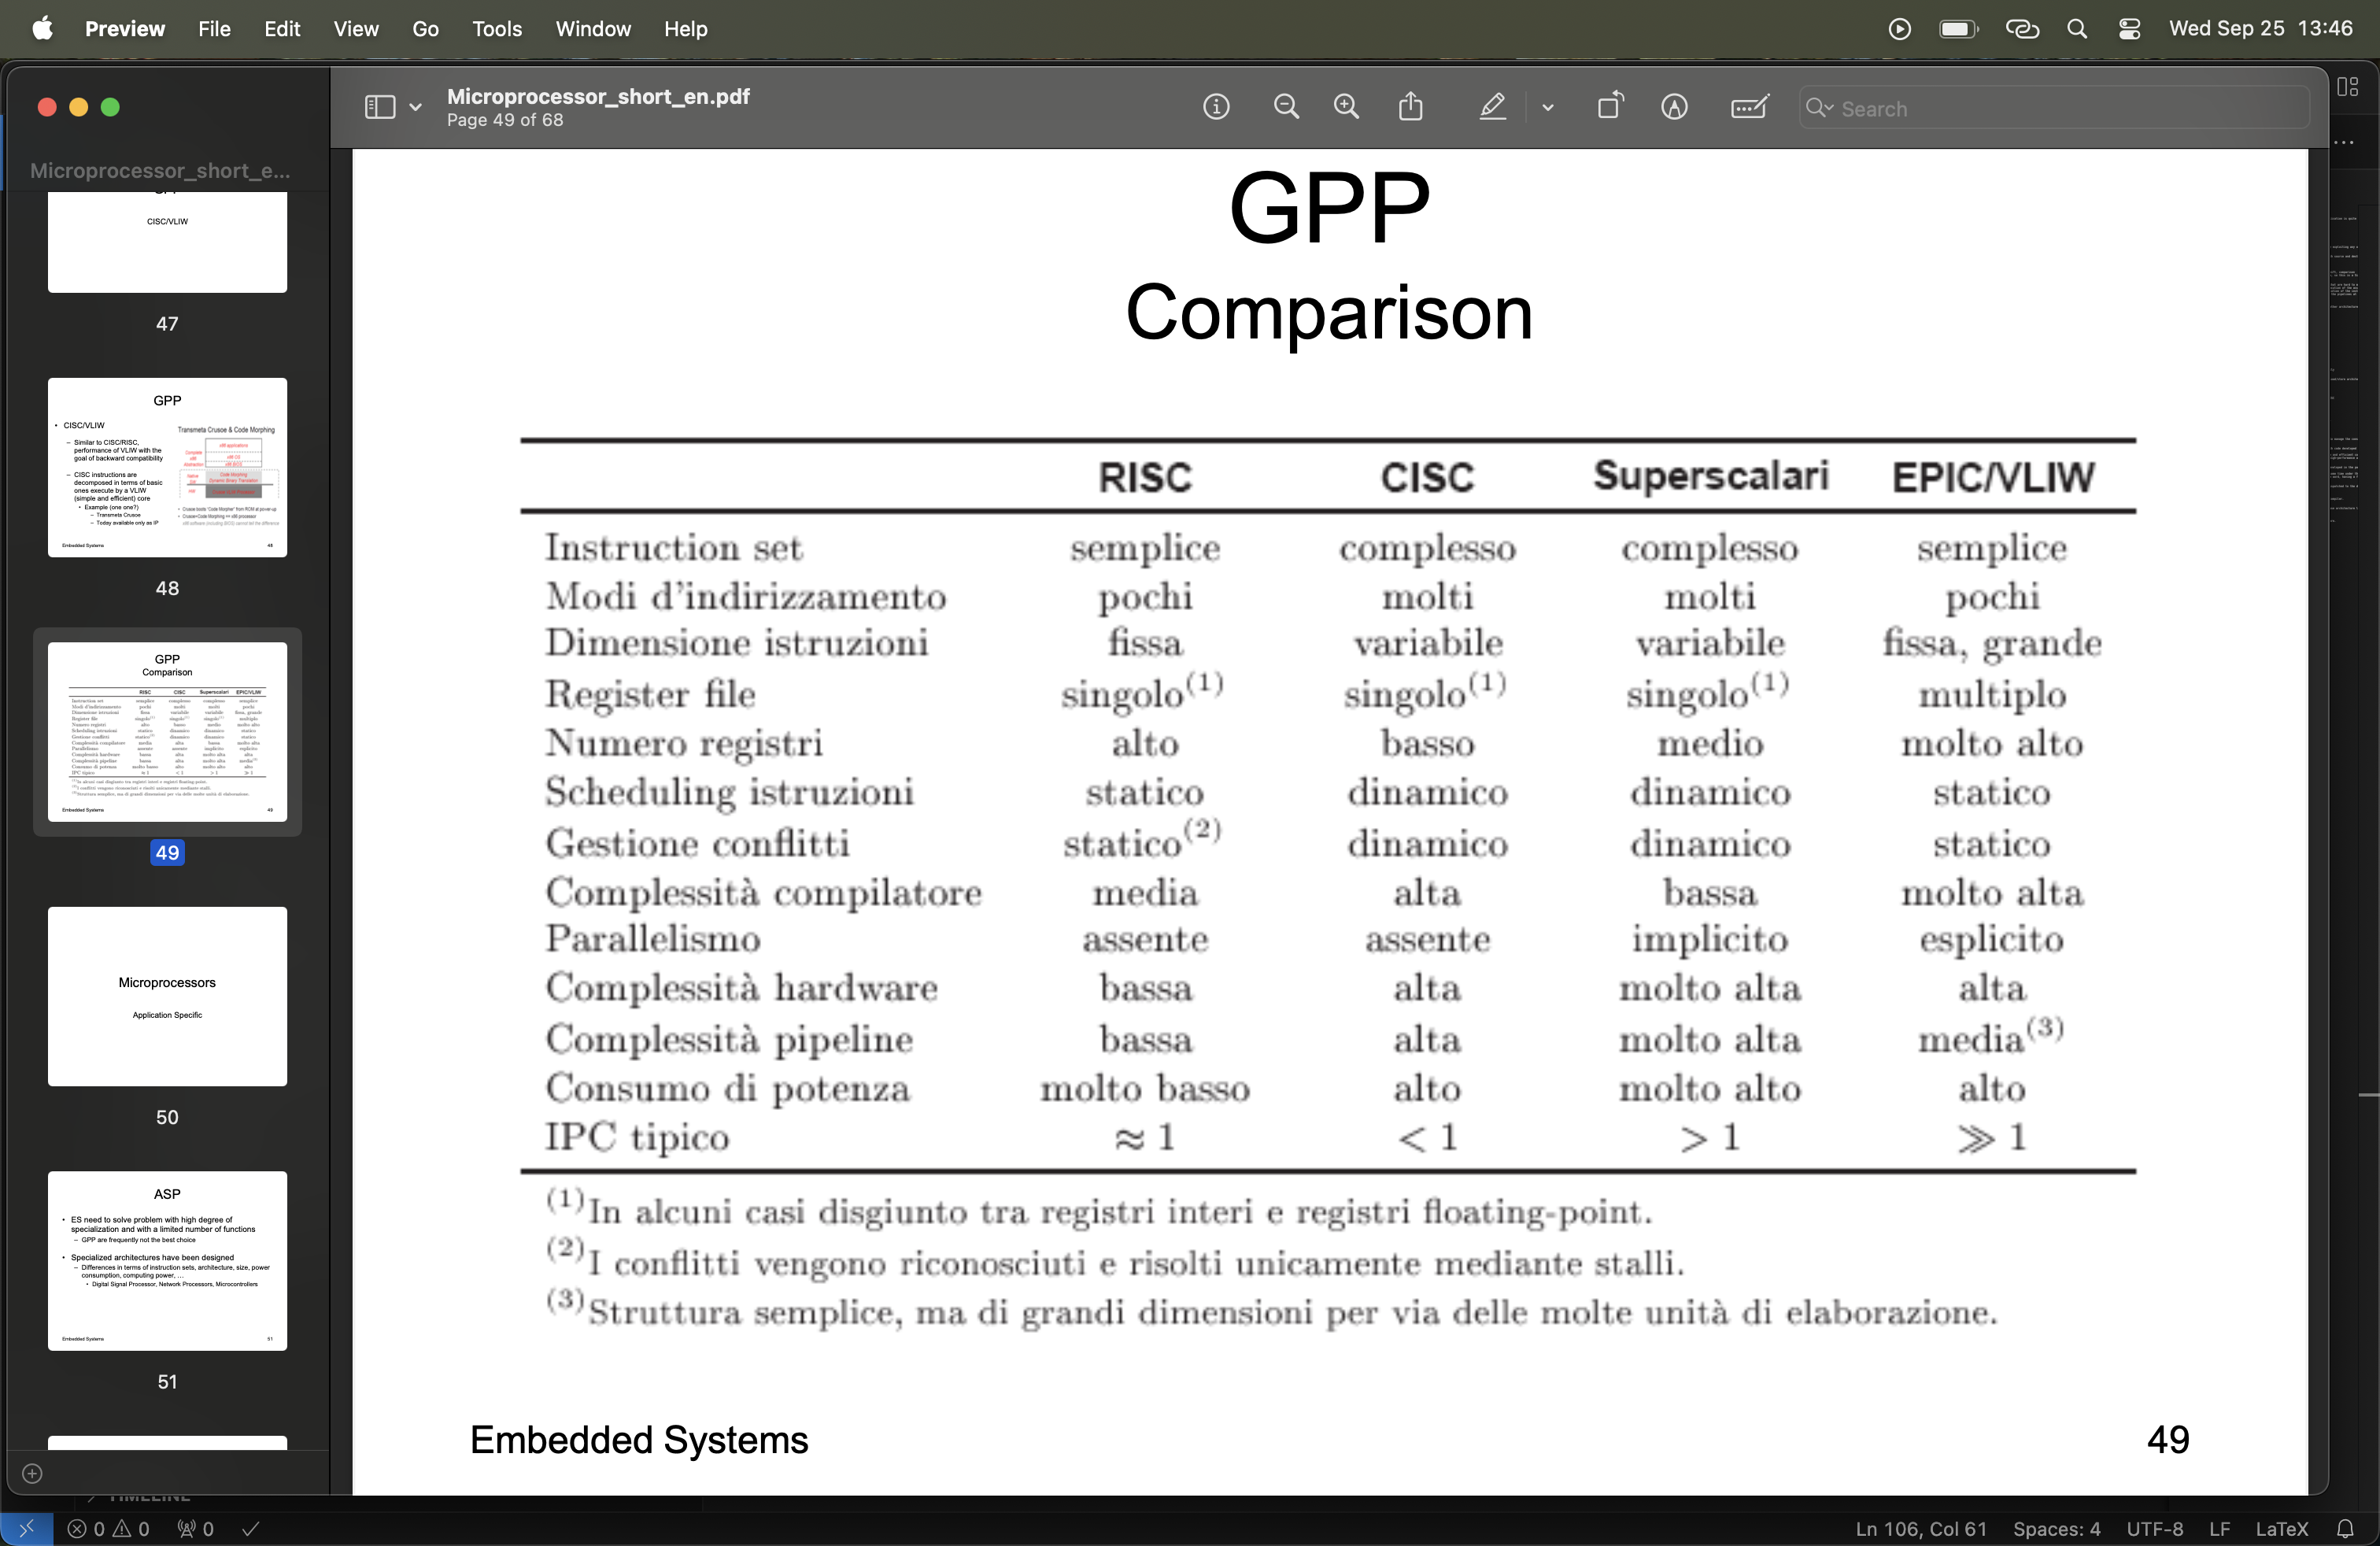
\includegraphics[width=0.75\linewidth]{images/comparison.png}
    \caption{Comp}
\end{figure}
